\documentclass[a4paper,12pt]{article}


\usepackage[MeX]{polski}
\usepackage[utf8]{inputenc}	% kodowanie znaków
\usepackage{indentfirst}

\usepackage{upquote}  	% zamiana cudzysłowów klasycznych (,, ") na górne (" ") w kodach źródłowych
\usepackage{graphicx}	% wstawianie obrazków
\usepackage{amsmath}
\usepackage{listings}


\def\PICSDIR{PICS}

% Ustawienie marginesów
\oddsidemargin=0.5cm
\evensidemargin=-0.5cm
\topmargin=0cm
\textwidth=16cm
\textheight=23cm

% Ładniejsze tabelki
\usepackage{booktabs}


\frenchspacing

\clubpenalty=10000		% to kara za sierotki
\widowpenalty=10000		% nie pozostawia wdów
\brokenpenalty=10000 	% nie dzieli wyrazów pomiędzy stronami


\sloppy

% Pakiety z ładnymi czcionkami
\usepackage[T1]{fontenc}
\usepackage{lmodern}


% Ładniejsze tabelki
\usepackage{booktabs}

% Ustawienia wyglądu listingów
\lstset{
	language=C++,                               % choose the default language of the code
	basicstyle=\footnotesize\ttfamily,       	% the size of the fonts that are used for the code
	numbers=left,                   		% where to put the line-numbers
%	numberstyle=\tiny,      			% the size of the fonts that are used for the line-numbers
	stepnumber=1,                   		% the step between two line-numbers. If it's 1 each line will be numbered
	numbersep=5pt,                  		% how far the line-numbers are from the code
	showspaces=false,               		% show spaces adding particular underscores
	showstringspaces=false,         	% underline spaces within strings
	showtabs=false,                 		% show tabs within strings adding particular underscores
	tabsize=4,	                		% sets default tabsize
	captionpos=b,                   		% sets the caption-position
	breaklines=true,                		% sets automatic line breaking
	breakatwhitespace=true,        	% sets if automatic breaks should only happen at whitespace
	extendedchars=true,
	keywordstyle=\bfseries,
	identifierstyle=,
	commentstyle=\slshape,
	stringstyle=\slshape,
	xleftmargin=30pt,
	frame=tb,
	framexleftmargin=30pt,
}

\begin{document}

\title{{\small Metody Bioinformatyki}\\Wykorzystanie PCA do analizy danych z mikromacierzy DNA}
\author{Maciej Czerniak, Marcin Kamionowski, Kacper Szkudlarek}

\maketitle

\begin{abstract}
Dokumentacja końcowa realizacji projektu z przedmiotu "Metody Bioinformatyki". W ramach projektu wykonane zostało oprogramowanie wykorzystujące metodę Analizy Składowych Głównych (PCA) do przetwarzania danych uzyskanych z mikromacierzy DNA oraz wygenerowanych danych testwych.
\end{abstract}


\section{Wstęp}
\textbf{Analiza głównych składowych} (ang. Principal Component Analysis, PCA) jest jedną ze statystycznych metod analizy czynnikowej. Zbiór danych składający się z N obserwacji, z których każda obejmuje K zmiennych, można interpretować jako chmurę N punktów w przestrzeni K-wymiarowej. Celem PCA jest taki obrót układu współrzędnych, aby maksymalizować w pierwszej kolejności wariancję pierwszej współrzędnej, następnie wariancję drugiej współrzędnej, itd.. Tak przekształcone wartości współrzędnych nazywane są ładunkami wygenerowanych czynników (składowych głównych). W ten sposób konstruowana jest nowa przestrzeń obserwacji, w której najwięcej zmienności wyjaśniają początkowe czynniki. PCA jest często używana do zmniejszania rozmiaru zbioru danych statystycznych, poprzez odrzucenie ostatnich czynników.

\textbf{Mikromacierz DNA} jest to płytka szklana lub plastikowa z naniesionymi w regularnych pozycjach mikroskopowej wielkości polami (ang. spots), zawierającymi różniące się od siebie sekwencją fragmenty DNA. Fragmenty te są sondami, które wykrywają przez hybrydyzację komplementarne do siebie cząsteczki DNA lub RNA.

\begin{figure}
\centering
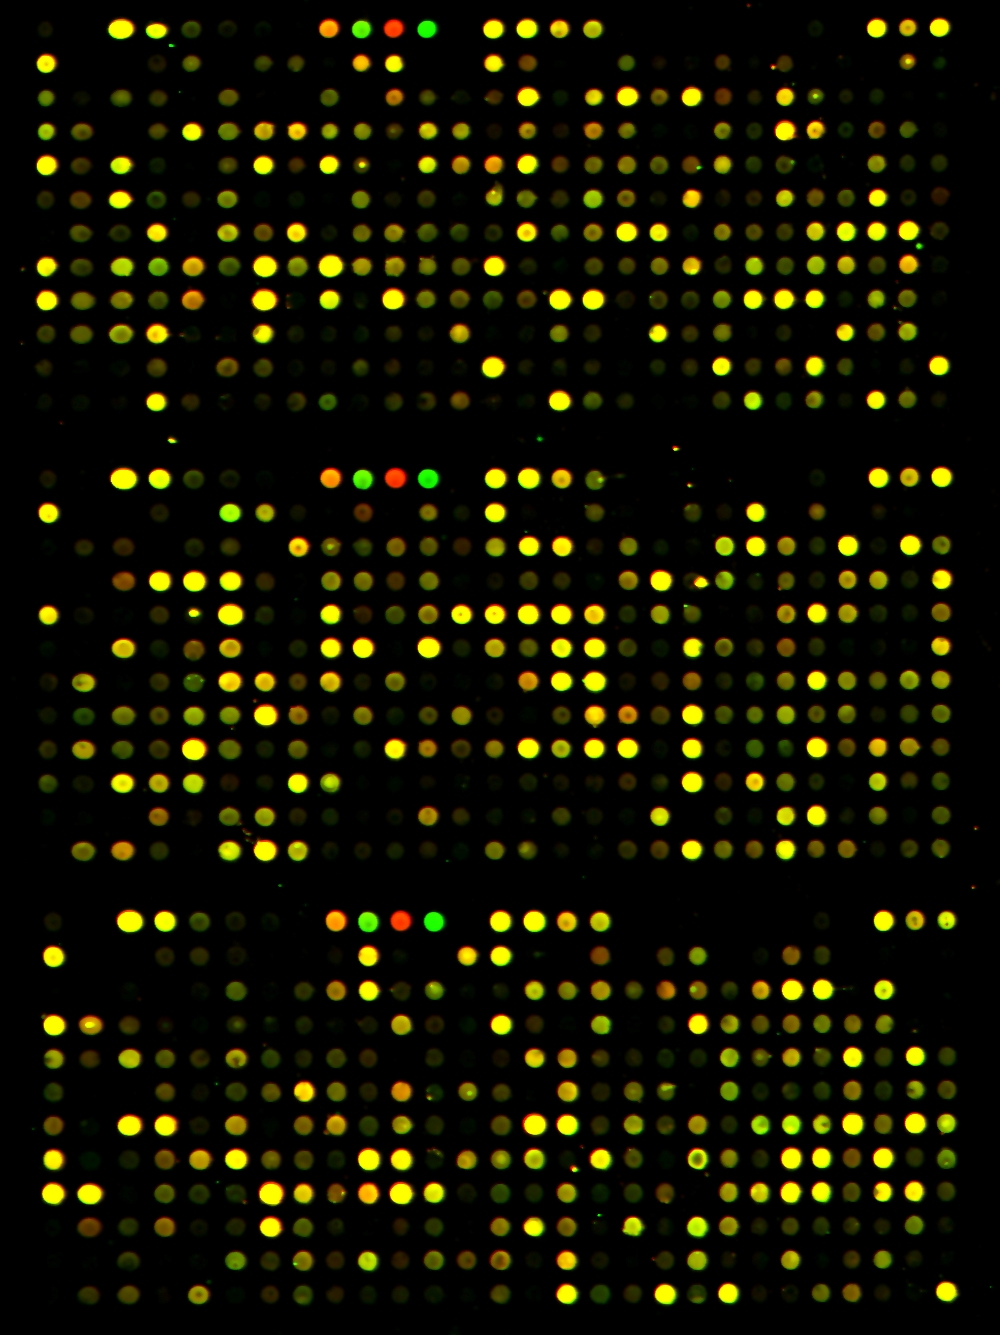
\includegraphics[width=5cm]{\PICSDIR/cDNA.jpg}
\caption{Pokolorowana próbka danych z mikromacierzy cDNA}
\label{rys:cDNA}
\end{figure}

Dane (Rys: \ref{rys:cDNA}) uzyskiwane w eksperymentach prowadzonych z wykorzystaniem mikromacierzy to wartości intensywności czerwonej oraz zielonej fluorescencji każdego z pół na płytce. Jedonorazowo w eksperymencie możliwe jest badanie ekspresji kilku tysięcy genów, dlatego uzyskane dane są wysoce złożone i wielowymiarowe.


\section{Wykonana implementacja}

Implementacja zgodnie z opisem zawartym w dokumentacji wstępnej została podzielona na kilka części:

\begin{enumerate}
\item Modułu wczytywania danych.

Dane do analizy dostarczone są do aplikacji w surowej postaci plików tekstowych (tabbed separate data). Przyjęty format analizowanych danych zakłada, że w kolumnach zostały oznaczone poszczególne przeprwaodzone eksperymetny, natomiast w wierszach znajdują się cechy, które poddane zosatną PCA.  Przy wczytywaniu użytkownik może wybrac jaki zakres danych ma być poddany analizie. Możliwe jest pominięcie pewnej ilości początkowych cech, a także wybranie zakresu eksperymentów, które maja być brane pod uwagę. Dane zostają wczytane do stryktury danych Mat z biblioteki OpenCV \cite{opencv}, która następnie przekazywana jest do analizy.
\item Stworzenie graficznego interfejsu użytkownika.

Interfejs graficzny został stworzonwy w oparciu o wieloplatformowa bibliotekę Qt \cite{qt}. Z poziomu interfejsu możliwe jest wczytywanie danych, wświetlenie błędu średniokwadratowego [CO JESZCZE? MOŻE START DODAĆ].

[OBRAZEK INTERFEJSU]

\item Moduł analizatory i przetwarzający dane wejściowe.

Analiza danych polega na poddaniu ich analizie składowych głównych (PCA). Wykorzysatanu został moduł PCA znajdująca się w bibliotece OpenCV. Dane podawane są w postaci struktury danych Mat i w takiej samej formie są zwaracane. Dane poddawane są także odwrotnemu PCA w calu odtworzenia oryginalnej macierzy. Dzięki temu możliwe staje się policzenie błedu średniokwadratowego. 

[OBRAZEK Z WYNIKAMI]

\item Moduł generatora danych

Dodatkowo w celu wygenerowania danych testowych stowrzony został moduł generatora. Generowne dane są opisem  jednostajengo prostolinowego ruchu obiektu w przestrzeni, widzianego z wielu punktów obserwacji (kamer). W celu wygenerowania danych należy podać pozycję początkową i końcowa ruchu, ilość i pozycję kamer, a także ilość przeprowadonych (co 1s) pomiarów. Wygeneroweane dane zapisywane są do plikutekstowego w postaci kompatybilnej z modułem wczytywania danych. 
\end{enumerate}

Całość implementacji została wykonana w języku C/C++ pod kontrolą systemu Linux. Dzięki użyciu multiplatformowych bibliotek (Qt, OpenCV) aplikacja jest w pełni przenośna. Uruchomienie programu na nowym systemie wymaga jedynie rekompilacji pod kontrolą tego systemu. Do synchronizacji pracy programistów w czasie tworzenia projhektu, użyty został rozproszony system wersjonowania plików Git. 
%
%\begin{itemize}
%\item Implementacja zostanie wykonana w języku C/C++ dla systemu Linux.
%\item Wykorzystanie biblioteki Qt do stworzenia GUI.
%\item Użycie gotowej implementacji PCA z pakietu OpenCV.
%\end{itemize}

\bibliographystyle{plplain}
\bibliography{mybib}{}

\end{document}
